\documentclass[tikz,border=2pt]{standalone}
\usepackage{amsmath}
\usepackage{pgfplots}
\pgfplotsset{compat=1.18}
\usetikzlibrary{arrows.meta}
\begin{document}
% Keys (Country, Year) of co2_total (x: 6 keys) and gdp (y: 5 keys); 4 keys in both (green),
% Netherlands 2020/2021 only in x (blue), France 2021 only in y (red); rows kept by inner (4), left (6), right (5), full (7).
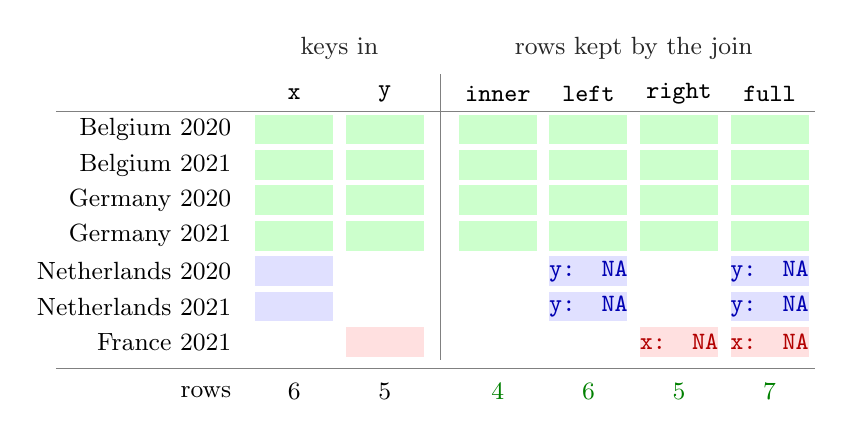
\begin{tikzpicture}[font=\small, >={Latex[length=2mm]},
  hd/.style={font=\small\ttfamily},
  na/.style={font=\small\ttfamily}]
  \def\h{0.45}
  \def\kB{b}\def\kL{l}\def\kR{r}
  \def\cw{1.15}
  \def\xo{2.45}
  % header
  \node[hd] at (\xo+0.5*\cw,0) {x};
  \node[hd] at (\xo+1.5*\cw,0) {y};
  \foreach \t [count=\j] in {inner,left,right,full}
    \node[hd] at (\xo+2.25*\cw+\j*\cw-0.5*\cw,0) {\t};
  \node[anchor=south, gray!30!black] at (\xo+\cw,0.32) {keys in};
  \node[anchor=south, gray!30!black] at (\xo+2.25*\cw+2*\cw,0.32) {rows kept by the join};
  % rows: label / class (b = both, l = left only, r = right only)
  \foreach \lab/\k [count=\i] in {Belgium 2020/b,Belgium 2021/b,Germany 2020/b,Germany 2021/b,Netherlands 2020/l,Netherlands 2021/l,France 2021/r} {
    \def\y{-\i*\h}
    \node[anchor=east] at (\xo-0.1,\y) {\lab};
    % key columns x and y
    \ifx\k\kB
      \fill[green!20] (\xo+0.08,\y+0.42*\h) rectangle (\xo+\cw-0.08,\y-0.42*\h);
      \fill[green!20] (\xo+\cw+0.08,\y+0.42*\h) rectangle (\xo+2*\cw-0.08,\y-0.42*\h);
      \foreach \j in {1,2,3,4}
        \fill[green!20] (\xo+1.25*\cw+\j*\cw+0.08,\y+0.42*\h) rectangle (\xo+2.25*\cw+\j*\cw-0.08,\y-0.42*\h);
    \fi
    \ifx\k\kL
      \fill[blue!12] (\xo+0.08,\y+0.42*\h) rectangle (\xo+\cw-0.08,\y-0.42*\h);
      \foreach \j in {2,4} {
        \fill[blue!12] (\xo+1.25*\cw+\j*\cw+0.08,\y+0.42*\h) rectangle (\xo+2.25*\cw+\j*\cw-0.08,\y-0.42*\h);
        \node[na, blue!70!black] at (\xo+1.75*\cw+\j*\cw,\y) {y: NA};
      }
    \fi
    \ifx\k\kR
      \fill[red!12] (\xo+\cw+0.08,\y+0.42*\h) rectangle (\xo+2*\cw-0.08,\y-0.42*\h);
      \foreach \j in {3,4} {
        \fill[red!12] (\xo+1.25*\cw+\j*\cw+0.08,\y+0.42*\h) rectangle (\xo+2.25*\cw+\j*\cw-0.08,\y-0.42*\h);
        \node[na, red!70!black] at (\xo+1.75*\cw+\j*\cw,\y) {x: NA};
      }
    \fi
  }
  % separators
  \draw[gray] (0,-0.5*\h) -- (\xo+6.25*\cw,-0.5*\h);
  \draw[gray] (\xo+2.12*\cw,0.25) -- (\xo+2.12*\cw,-7.5*\h);
  % totals
  \node[anchor=east] at (\xo-0.1,-8.4*\h) {rows};
  \foreach \n [count=\j] in {6,5} \node at (\xo+\j*\cw-0.5*\cw,-8.4*\h) {\n};
  \foreach \n [count=\j] in {4,6,5,7} \node[green!50!black] at (\xo+1.75*\cw+\j*\cw,-8.4*\h) {\n};
  \draw[gray] (0,-7.75*\h) -- (\xo+6.25*\cw,-7.75*\h);
\end{tikzpicture}
\end{document}
